\section{Hardware}
Perangkat keras komputer adalah komponen fisik atau komponen komputer, seperti monitor, keyboard, penyimpanan data komputer, kartu grafis, kartu suara dan motherboard. \cite{clements2006principles} Sebaliknya, perangkat lunak adalah instruksi yang bisa disimpan dan dijalankan oleh perangkat keras.
Perangkat keras diarahkan oleh perangkat lunak untuk menjalankan perintah atau instruksi apapun. Kombinasi perangkat keras dan perangkat lunak membentuk sistem komputasi yang dapat digunakan
\subsection{Arsitektur Von Neumann}
Kerangka untuk semua komputer modern adalah arsitektur Von Neumann seperti pada gambar \ref{vonneumann}, yang dirinci dalam makalah tahun 1945 oleh matematikawan Hungaria John von Neumann. Ini menggambarkan arsitektur desain untuk komputer digital elektronik dengan subdivisi unit pemrosesan yang terdiri dari unit logika aritmetika dan register prosesor, unit kontrol yang berisi register instruksi dan penghitung program, memori untuk menyimpan data dan instruksi, penyimpanan massa eksternal, dan mekanisme input dan output. \cite{von1945first}
\centerline{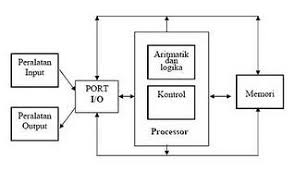
\includegraphics[width=1\textwidth]{figures/vonneumann.JPG}}
	\caption{Skema Von Neumann}
	\label{VonNeumann}
	\end{figure}
Arti dari istilah tersebut telah berevolusi untuk berarti komputer program tersimpan dimana pengambilan instruksi dan operasi data tidak dapat terjadi pada saat yang bersamaan karena mereka memiliki bus umum. Ini disebut sebagai bottleneck Von Neumann dan sering membatasi kinerja sistem. \cite{markgrafneumann}

